\section{The Proof-of-Anonymous-Stake (PoAS) protocol}
This section introduces a new staking algorithm that was introduced to the
Spectrecoin mainnet through the release of v3.0.9 and a hard-fork on
17\textsuperscript{th} May 2019. This is the first known implementation
of a private staking protocol employing ring-signatures in the staking
transactions. This protocol was designed and coded by Spectrecoin lead
developer Philip Mueller (\textit{@Tek}). The protocol is based on the
PoSv3 protocol that we described in the previous section.



\subsection{Introduction}
We consider that a privacy focused pure Proof-of-Stake (\textit{PoS})
network such as Spectrecoin needs to be able to maintain consensus through
a mechanism that maintains privacy, prevents easy blockchain analysis and
is censorship resistant. Hence, such a network is not complete without a
way to stake in private. There should be a way to maintain the privacy of
all the network participants throughout the staking process. The
participants should also be able to acquire their stake reward whilst
maintaining their privacy.



\subsection{The Problem}

In a standard staking transaction (\textit{PoSv3}) a value known as the
'\textit{kernel hash}' is calculated from several inputs including values
taken from the last valid block, called a '\textit{StakeModifier}' and
the value of the user's UTXO. A valid '\textit{kernel hash}' needs to be
below a certain threshold that is determined by a separate calculation.
The user (\textit{the wallet}) who is able to generate a valid
'\textit{kernel hash}' will be granted the right to add the next block
to the block-chain. The newly added block includes the generated stake
reward (XSPEC) and any transactions currently in the memory pool + any
fees. The UTXO used to calculate the valid '\textit{kernel hash}' will
be spent and the generated stake reward + the value of the spent UTXO
will be included in a newly generated UTXO associated with the same public
address. In this way every stake that has been generated as a result of
UTXOs associated with a certain public address will forever be linked to
that address and it's plain for all to see. Below is an example of a
standard staking transaction\footnote{https://chainz.cryptoid.info/xspec/block.dws?1190944.htm}:



\begin{figure}[h]
    \centering
    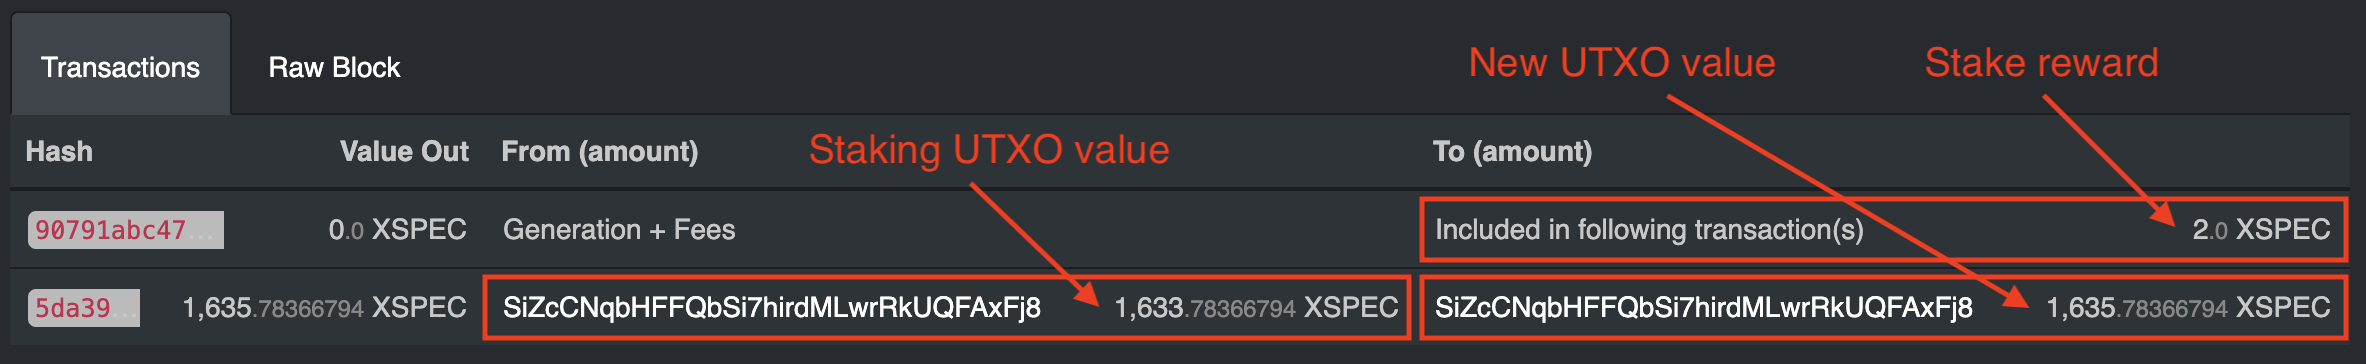
\includegraphics[width=\textwidth]{Images/txnexample.png}
    \caption{Example of a staking transaction}
    \label{fig}
\end{figure}


\noindent
As with any typical PoS cryptocurrency the staking transactions suffer
from all the privacy issues of a standard UTXO transaction, and these
transactions are potentially traceable and linkable on the blockchain.
It would therefore require some effort from the users to try to maintain
anonymity in a standard PoS system and that will in turn weaken the overall
resilience of the network against analysis. The network should not have to
depend on the participants to maintain anonymity. All the staking
transactions completed by the same user can potentially be linked and users’
balances can be estimated, hence the ‘\textit{rich list}’ feature of many
block explorers. As explained previously, most block-chain forensic analysis
focuses on address re-use and change addresses and this is exactly what you
get with a standard PoS network.



\subsection{The Solution}
We have therefore developed what we call ‘\textbf{\textit{Proof-of-Anonymous-Stake}}’
(PoAS) to solve this problem. This is a brand new and novel staking protocol
utilising only SPECTRE and ring-signatures in the staking transactions and
the rewards are also paid in SPECTRE. This offers a through-and-through
confidential way to maintain consensus and provide strong privacy for
participants whilst securing the network. It is also appropriate to emphasise
that this confidential and private consensus mechanism is totally
decentralised and does not depend on any central servers or authority and is
100\% peer-to-peer and there is no trusted setup. This provides very strong
network resilience with no single point of failure.

\begin{figure}[h]
	\centering
	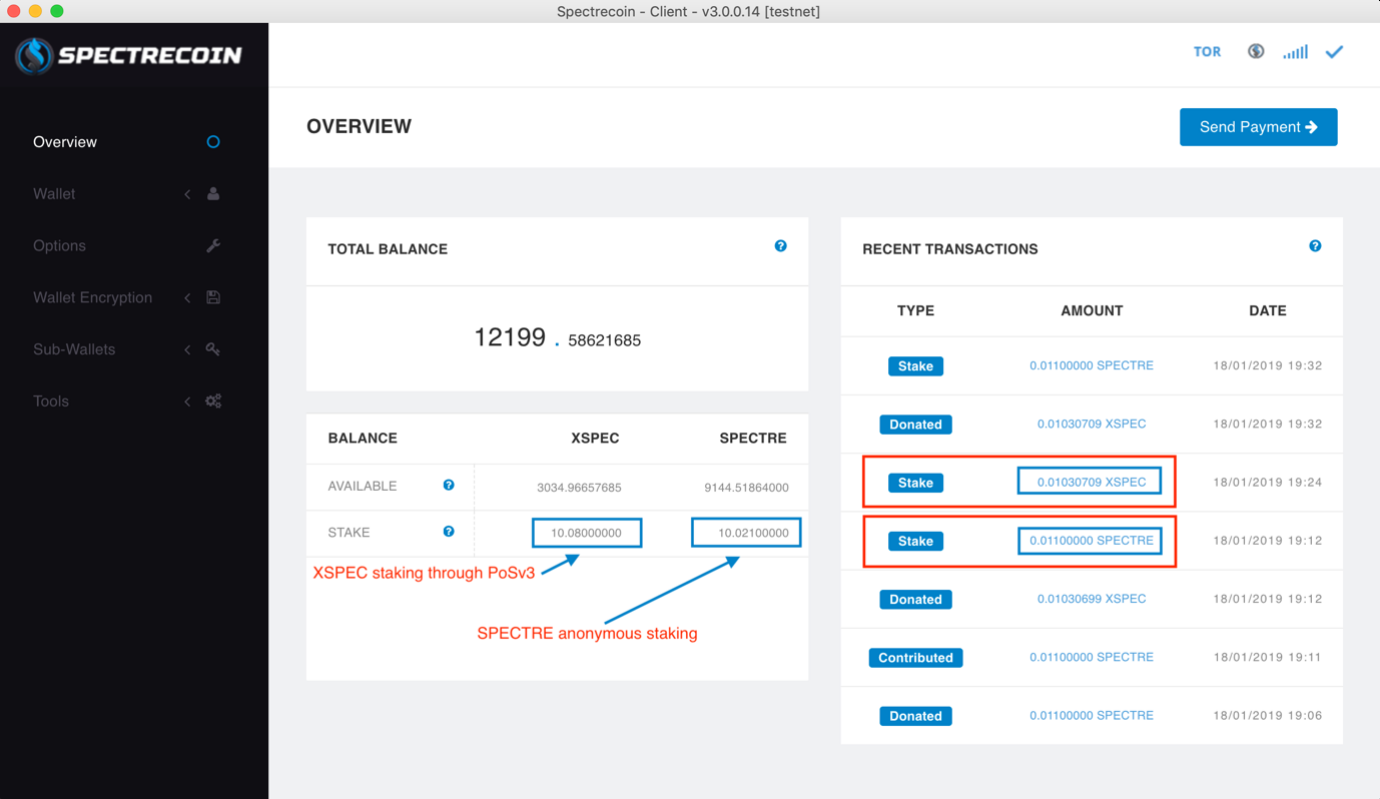
\includegraphics[width=\textwidth]{WalletUI-3x.png}
	\caption{New updated UI for the Spectrecoin wallet in v3.x}
\end{figure}



\subsection{Benefits of Anonymous Staking}
The benefits are straight forward and easy to appreciate; if you transfer
your holdings to \textit{SPECTRE}, our anonymous coin, nobody will be able
to know your balance, nobody will know how much you stake and if you keep
transactions \textit{SPECTRE $<>$ SPECTRE} you preserve your privacy at all
times. It is useful however to remember that once SPECTRE is converted to
XSPEC all your \textit{XSPEC $<>$ XSPEC} transactions are again potentially
traceable. Note that the potential traceability only becomes an issue
\underline{after} the conversion from SPECTRE $>>$ XSPEC and does not affect
the previous SPECTRE transaction.
\newpage
\noindent
With the addition of anonymous staking to Spectrecoin and the updated UI it
is now easy to distinguish between the different transactions and you will
clearly see if you are staking XSPEC, SPECTRE or both. The previously
described ‘\textit{Development Contribution Blocks}’ (marked as ‘contributed’)
will still occur every 1 in 6 blocks regardless of whether the block has
been staked via the standard staking transaction or the anonymous ATXO
staking transaction.
\\
\\
\noindent
In addition to the pre-programmed 1/6 ‘\textit{Development Contribution Blocks}’,
you can still choose to donate extra via the ‘\textit{Options}’ menu in the wallet.



\subsection{PoAS Implementation Detail}
In Spectrecoin's PoAS the basic structure of the staking transactions and
the rules remain mainly intact. But, instead of using the UTXO transaction
hash as an input in the '\textit{kernel hash}' calculation and the
difficulty calculations, the so called '\textit{keyimage}' associated with
an ATXO is used instead as an input to calculate the '\textit{kernel hash}'
and difficulty. An ATXO is an '\textit{Anonymous Transaction Output}' and
associated with a discreet SPECTRE value. SPECTRE takes on discreet values,
like 100, 50, 40, 10, 1, 0.5 and so on. Each ATXO has a unique
cryptographically determined '\textit{keyimage}' associated with it.
\\
\\
\noindent
This '\textit{keyimage}' can be used to prevent double spend and once an
ATXO is spent the '\textit{keyimage}' is stored on the blockchain. The ATXO
is totally dissociated from any user and as each and every ATXO is a unique
'\textit{data-entity}', ATXOs cannot be linked to each other. Only the user
holds the '\textit{secret}' key needed to prove ownership and no information
is written to the block-chain that can in any way identify the owner of an
ATXO.
\\
\\
\noindent
In order to spend an ATXO or to use an ATXO in the staking transaction a user
need to provide a valid ring-signature with a ring size of 10. The staking
transaction therefore uses an ATXO as an input with 9 additional mixins for
the ring-signature and new ATXOs are generated to the value of the stake
reward in discreet units.



\subsubsection{ATXO staking logic}
Below is a summary of the logic for ATXO based staking w/ ring signatures.
\\
\\
\noindent
\underline{An ATXO staking transaction is valid, if:}
\begin{itemize}
	\item The transaction is PoSv3 compliant
	\item VIN[0] has a valid ring-signature of MIN\_RING\_SIZE 10 (must has ring size 10)
	\item The ‘\textit{keyImage}’ of the ATXO to be consumed is unspent (\textit{not the mixins})
	\item All ring-signature ATXOs meets minDepth maturity requirement
	\item The kernel hash calculated is below target
\end{itemize}
\newpage



\subsubsection{ATXO coinstake kernel protocol}
The coinstake kernel (input 0) must meet hash target according to the formula:



\vspace{5mm} %5mm vertical space
$ hash(nStakeModifier + keyImage + nTime) < bnTarget * nWeight  $
\vspace{5mm} %5mm vertical space

\noindent
This ensures that the chance of getting a coinstake is proportional to
the amount of coins one owns.
\\
\\
\noindent
\underline{The reason this hash is chosen is the following:}
\begin{itemize}
	\item nStakeModifier: scrambles computation to make it very difficult
	to precompute future proof-of-stake.
	\item nStakeModifier is either the UTXO hash (PoSv3) or keyImage (PoAS) 
	used for the last staking transaction plus the previous block's stake 
	modifier.
	\item keyImage: the keyImage of the ATXO used for staking is unique 
	regardles the mixins, makes sure an ATXO can only be used once for 
	generating a kernel hash.
	\item nTime: current timestamp.
\end{itemize}



\subsection{ATXO Splitting}
If an ATXO is staked, the algorithm searches for the denomination with the
least amount of unspent in the range of  $>= BASE\_FEE * 10$ and $<$ staked
ATXO value. If a denomination in this range is found with less than 100
unspent ATXOs, the staked ATXO will be split to create one ATXO of the
"\textit{low running}" denomination.
\\
\\
\noindent
Please see the examples below taken from the Spectrecoin Block explorer:

\begin{figure}[ht]
	
	\centering
	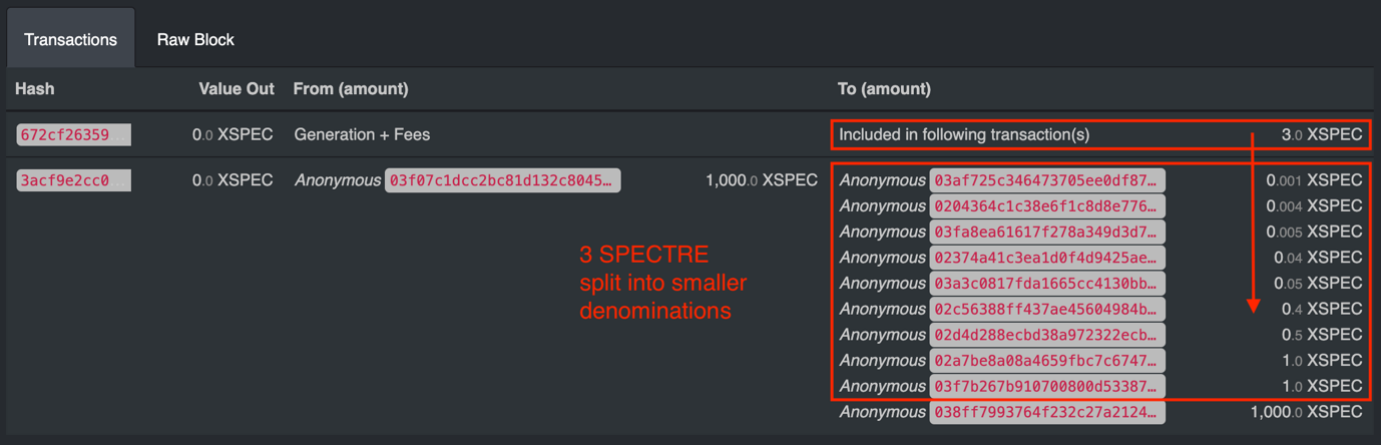
\includegraphics[width=\textwidth]{SPECTRE-StakeExample01.png}
	\caption{1000 SPECTRE is staked, 3 SPECTRE is staking reward for the 
	block, 0.001 SPECTRE is the lowest running and hence 3 SPECTRE gets 
	split into $0.001 + 0.004 + 0.005 + 0.04 + 0.05 + 0.4 + 0.5 + 1 + 1 = 3$ SPECTRE}
	\footnote{https://chainz.cryptoid.info/xspec/block.dws?1169499.htm}
\end{figure}



\begin{figure}[ht]
	\centering
	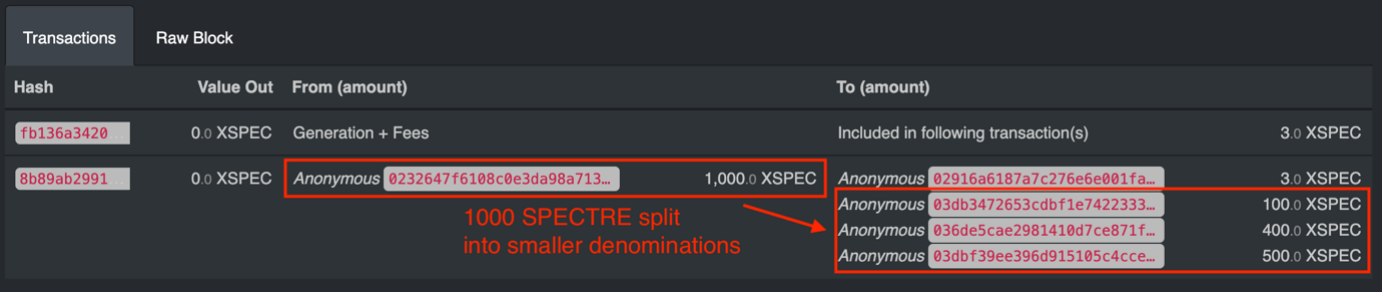
\includegraphics[width=\textwidth]{SPECTRE-StakeExample02.png}
	\caption{A further example of where 1000 SPECTRE is staked, 3 SPECTRE 
	is the staking reward for the block, 100 SPECTRE is the lowest running 
	and hence 1000 SPECTRE gets split into $100 + 400 + 500 = 1000$ SPECTRE}
	\footnote{https://chainz.cryptoid.info/xspec/block.dws?1168976.htm}
\end{figure}



\subsection{ATXO Consolidation}
Through the ‘\textit{Stealth Staking}’ process and in any SPECTRE $<>$
SPECTRE transactions there will be constant creation of small value ATXOs
from staking rewards and transaction change. This will tend to result in
larger transaction sizes in subsequent transactions as the number of
smaller value ATXOs are combined for the desired output amount.
\\
\\
\noindent
To solve this problem an extra ATXO ‘\textit{consolidation algorithm}’
has been implemented as part of the ATXO staking transaction where same
value ATXOs are consolidated into larger value ATXOs. After a valid
‘\textit{Kernel Hash}’ is found, the ATXO used for staking is added
as the first VIN to the transaction. The ‘\textit{consolidation algorithm}’
then tries to consolidate up to 50 ATXOs. The ATXOs are iterated from the
lowest to the highest amount with a maximum ATXO value to be consolidated
of 100 SPECTRE (MAX\_STAKING\_OUTPUT / 10). Every time 10 ATXOs are found
with same value they are added as an additional input. A maximum of 50
Inputs are added. In the below example we have chosen some values as an
illustration.



   \begin{table}[h]
	\centering
	\begin{tabular}{lllll}
		\textbf{Multiple} &     & \textbf{ATXO value} &      & \textbf{Consolidated ATXO value} \\
		10                & $*$ & 0.00000001          & $>>$ & 0.0000001 \\
		10                & $*$ & 3                   & $>>$ & 30        \\
		30                & $*$ & 1                   & $>>$ & 30        \\
	\end{tabular}

	\caption{Consolidation examples}
	\label{tbl:consolidationExamples}
	% Link to this label with \ref{tbl:consolidationExamples}
\end{table}

\noindent
The new consolidation algorithm ensures that at least 200 unspent
‘\textit{mixins}’ of any denomination remain. This means that if less
than 200 unspent ATXOs of a certain denomination exist, there is no
consolidation of that particular denomination. This serves a dual purpose;
it reduces the number of small value ATXOs and so reduces the subsequent
transaction sizes as discussed above, but it also works to increase what
we can call the ‘\textit{transactional entropy}’ of the network to reduce
the possibility of blockchain analysis by linking ATXOs in transactions.
It is apt at this stage to remember that each of the ATXOs whether
consolidated or not can all act as ‘\textit{mixins}’ in all future
transactions, and an observer can NEVER establish if the ATXO value has
been spent. Consequently, what we call the ‘\textit{Transactional Entropy}’
increases by the block with minimal blockchain bloat.
\newpage


\noindent
Please see the examples below taken from the Spectrecoin Block explorer:



\begin{figure}[ht]
	\centering
	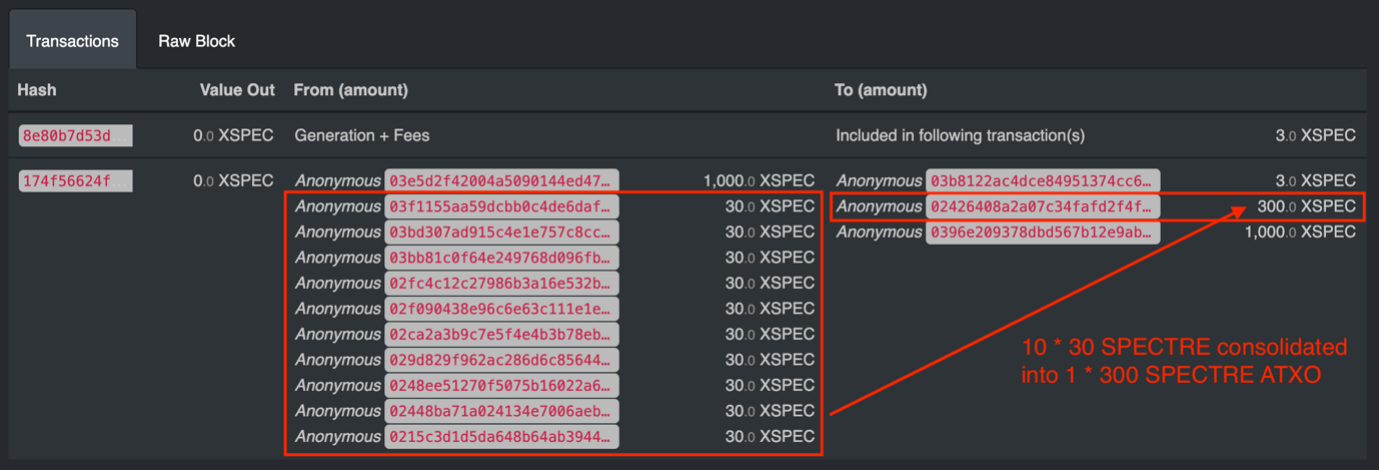
\includegraphics[width=\textwidth]{SPECTRE-ConsolidationExample01.png}
	\caption{In this example you can see $10 * 30$ SPECTRE being consolidated 
	into $1 * 30$ SPECTRE}
	\footnote{https://chainz.cryptoid.info/xspec/block.dws?1190841.htm}
\end{figure}
\begin{figure}[ht]
	\centering
	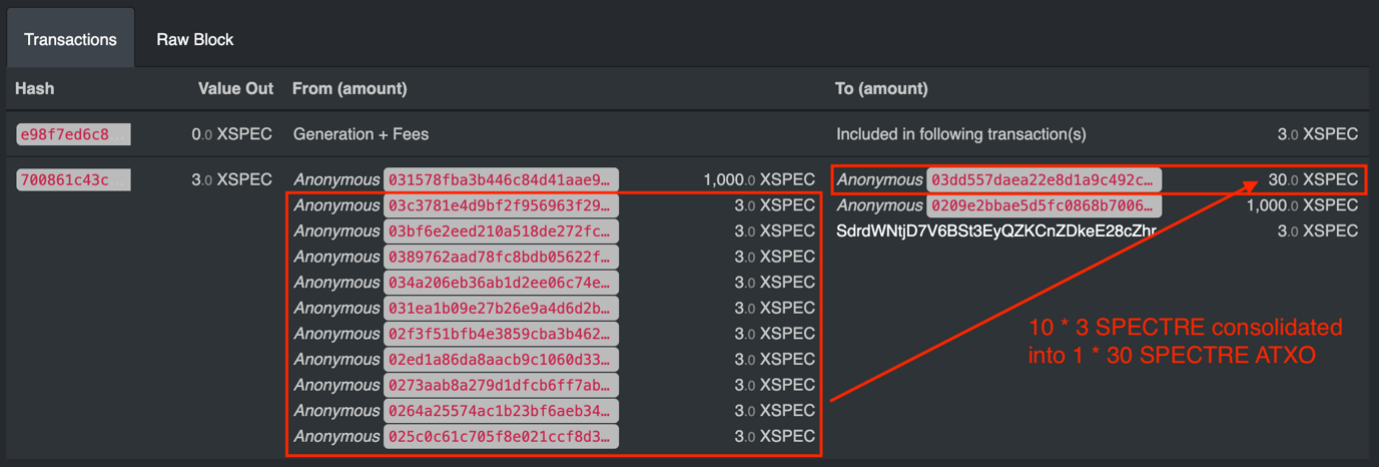
\includegraphics[width=\textwidth]{SPECTRE-ConsolidationExample02.png}
	\caption{In this example you can see $10 * 30$ SPECTRE being consolidated 
	into $1 * 30$ SPECTRE}
	\footnote{https://chainz.cryptoid.info/xspec/block.dws?1190898.htm}
\end{figure}



